\question An experimental setup consists of two large plates holding equal and opposite charge, with a uniform magnetic field of magnitude 0.3 T in between them which points into the page(see the figure). The plates are a distance $d=2$ cm apart.

 You fire a proton from the left with velocity $v=700$ m/s and observe that the proton passes through the plates undeflected. Next, you fire an electron from the left with a velocity of $v=650$ m/s, and observe that the electron drifts towards the top plate (as shown). What is the electric potential of the top plate relative to the bottom plate ($V_{top}-V_{bottom}$)?
\begin{figure}[ht!]
	\centering
	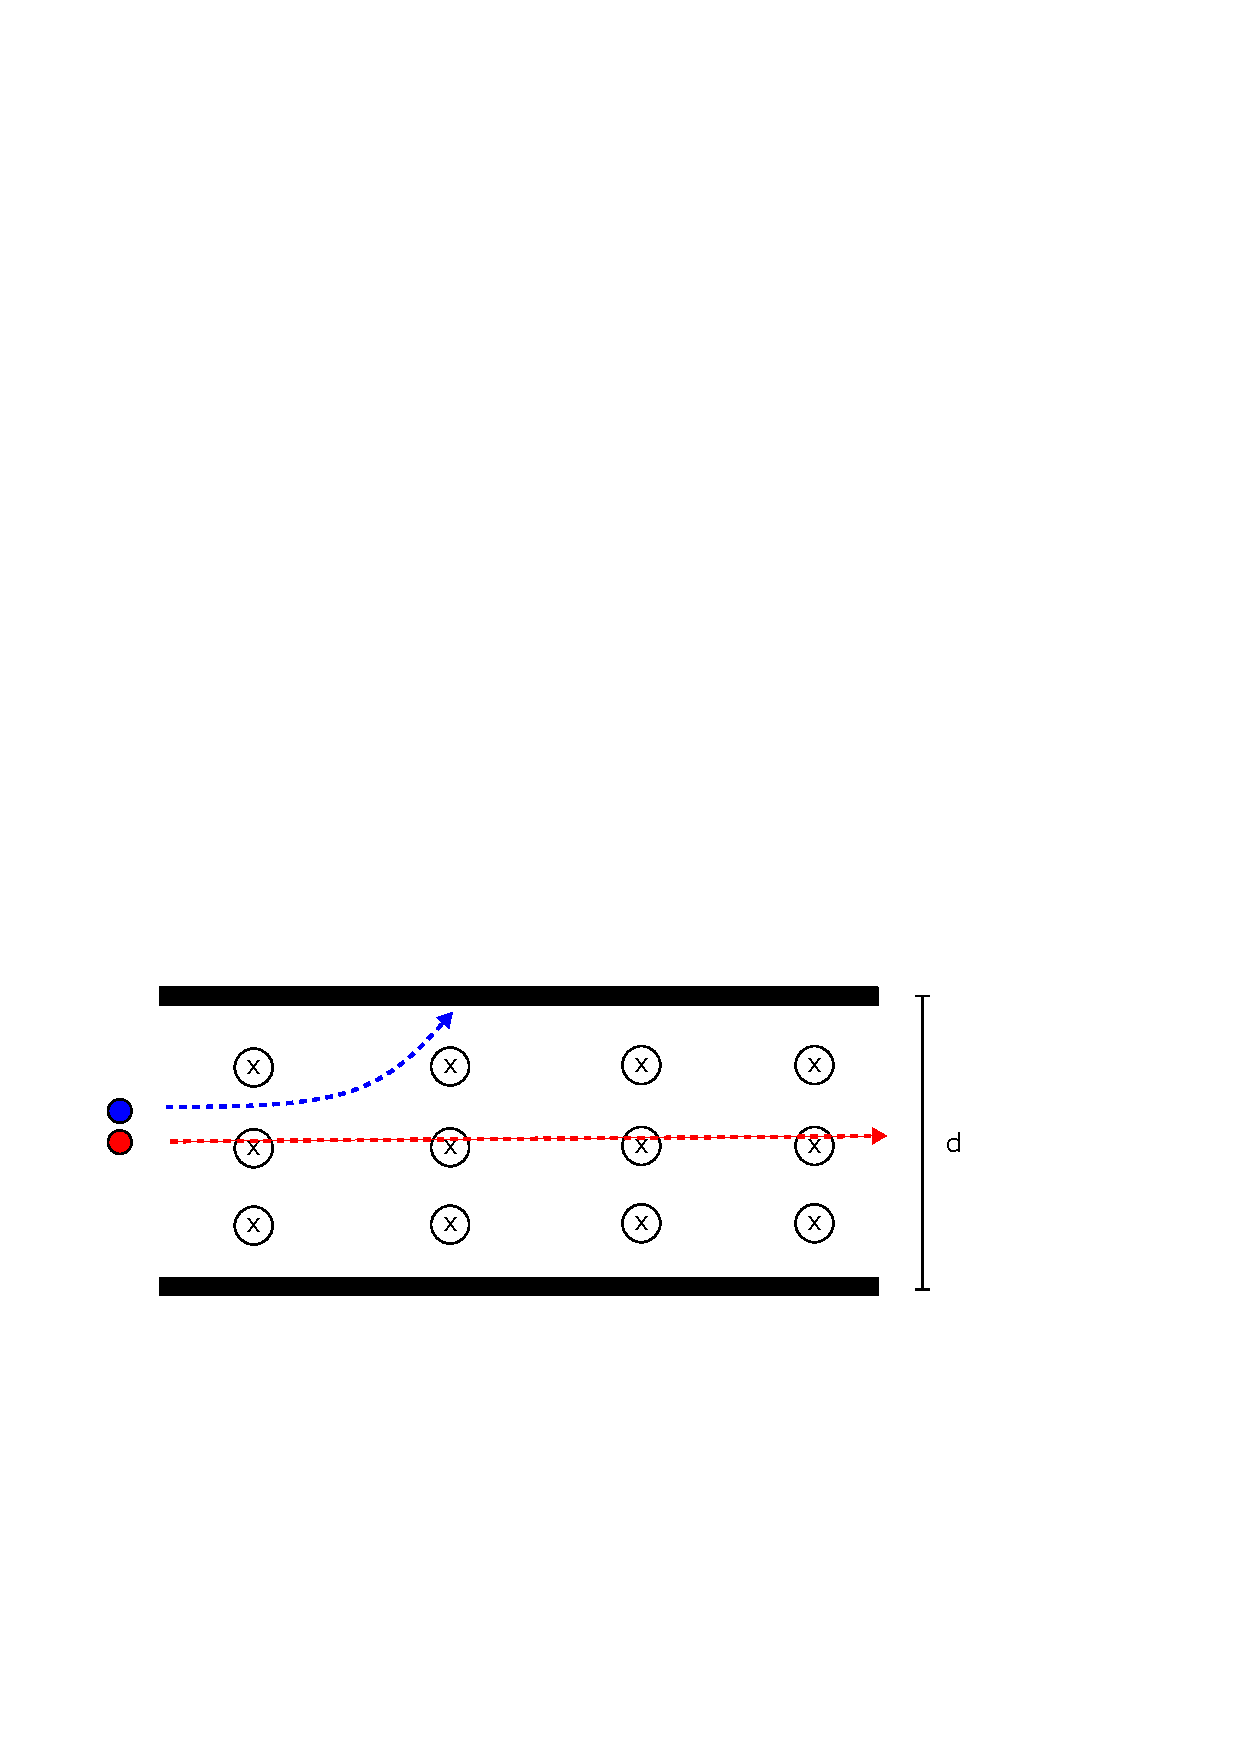
\includegraphics[width=10cm]{lorentz}
\end{figure}